% !TeX root = ../praktikum.tex
% !TeX encoding = UTF-8
% !Tex spellcheck = de_DE

Im Folgenden sollte nun die Temperaturabhängigkeit des Quanten-Hall- und des Shubnikov-de Haas-Effekts überprüft werden. Ziel dabei war es, die Grenztemperatur zu finden, bis zu welcher die beiden Effekte noch zu beobachten sind. 
Dazu wurden Messungen für unterschiedliche Temperaturwerte an der Probe aufgenommen. Begonnen wurde dabei bei der Ausgangstemperatur von \unit[2]{K} und es wurden in unregelmäßigen Intervallen Temperaturen bis hin zu \unit[40]{K} gewählt. Für jede Messung wurde analog zu den vorangegangenen Versuchsteilen das Magnetfeld mit einer Geschwindigkeit von \unitfrac[1]{T}{min} zwischen $-7,7$ und \unit[7,7]{T} gefahren. Auch hier wurde aufgrund der deutlicheren Hall-Plateaus in den Graphen weiterhin die Wechselstromquelle genutzt.


\begin{figure}[h]
	\centering
	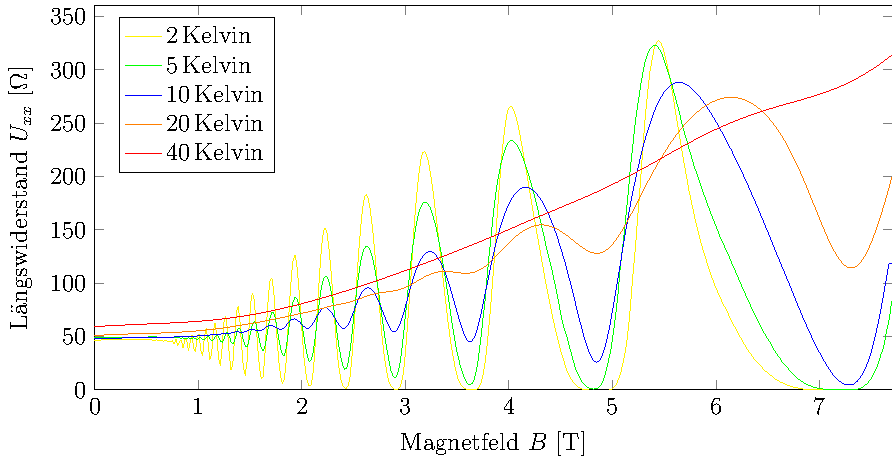
\includegraphics[scale=1]{graphs/temperatur/full_range.pdf}
	\caption[Hall-Widerstand unter Temperaturvariation]{
		Teilverlauf des berechneten Längswiderstands bei Unterschiedlichen Temperaturen. Für die Übersichtlichkeit wurde die Hälfte mit negativen Magnetfeldern nicht dargestellt.
	}
	\label{fig:temp_mess}
\end{figure}

In Abbildung~\ref{fig:temp_mess} ist jene Hälfte der Messergebnisse zu sehen, die bei positiven Magnetfeldern aufgenommen wurde.